\documentclass[xcolor=table,dvipsnames]{beamer}

\usepackage{lscape, amsmath, amsfonts, amssymb, setspace, theorem, wrapfig, graphicx, float, multirow, subfig, color, rotating, multicol, datetime, natbib, venndiagram, pstricks, xkeyval, tikz, etoolbox, verbatim}

\usepackage{listings}
\usepackage{xcolor}
 
\definecolor{codegreen}{rgb}{0,0.6,0}
\definecolor{codegreengray}{rgb}{0,0.4,0}
\definecolor{codegray}{rgb}{0.5,0.5,0.5}
\definecolor{codeblue}{rgb}{0.00,0,0.82}
\definecolor{backcolour}{rgb}{0.95,0.95,0.92}
\definecolor{jeopardy}{rgb}{.24,.47,.914}

\lstdefinestyle{mystyle}{
    backgroundcolor=\color{backcolour},   
    commentstyle=\color{codegreengray},
    numberstyle=\tiny\color{codegray},
    stringstyle=\color{codegreen},
    basicstyle=\ttfamily\footnotesize,
    breakatwhitespace=false,         
    breaklines=true,                 
    captionpos=b,                    
    keepspaces=true,                 
    numbers=left,                    
    numbersep=5pt,                  
    showspaces=false,                
    showstringspaces=false,
    showtabs=false,                  
    tabsize=2
}
 
\lstset{style=mystyle}

\title{GV300 - Quantitative Political Analysis}
\subtitle{University of Essex - Department of Government}
\date{Week 20 -- 10 February, 2020}				% or you can specify a date, just write it down instead of "\today"
\author{Lorenzo Crippa} 

\usetheme[progressbar=frametitle]{metropolis}
\usecolortheme{seahorse}						% try others: wolverine; crane...


\begin{document}

\begin{frame}[plain]
\begin{center}
\titlepage
\end{center}
\end{frame}

\begin{frame}{Question 1}
\begin{figure}[H]\centering
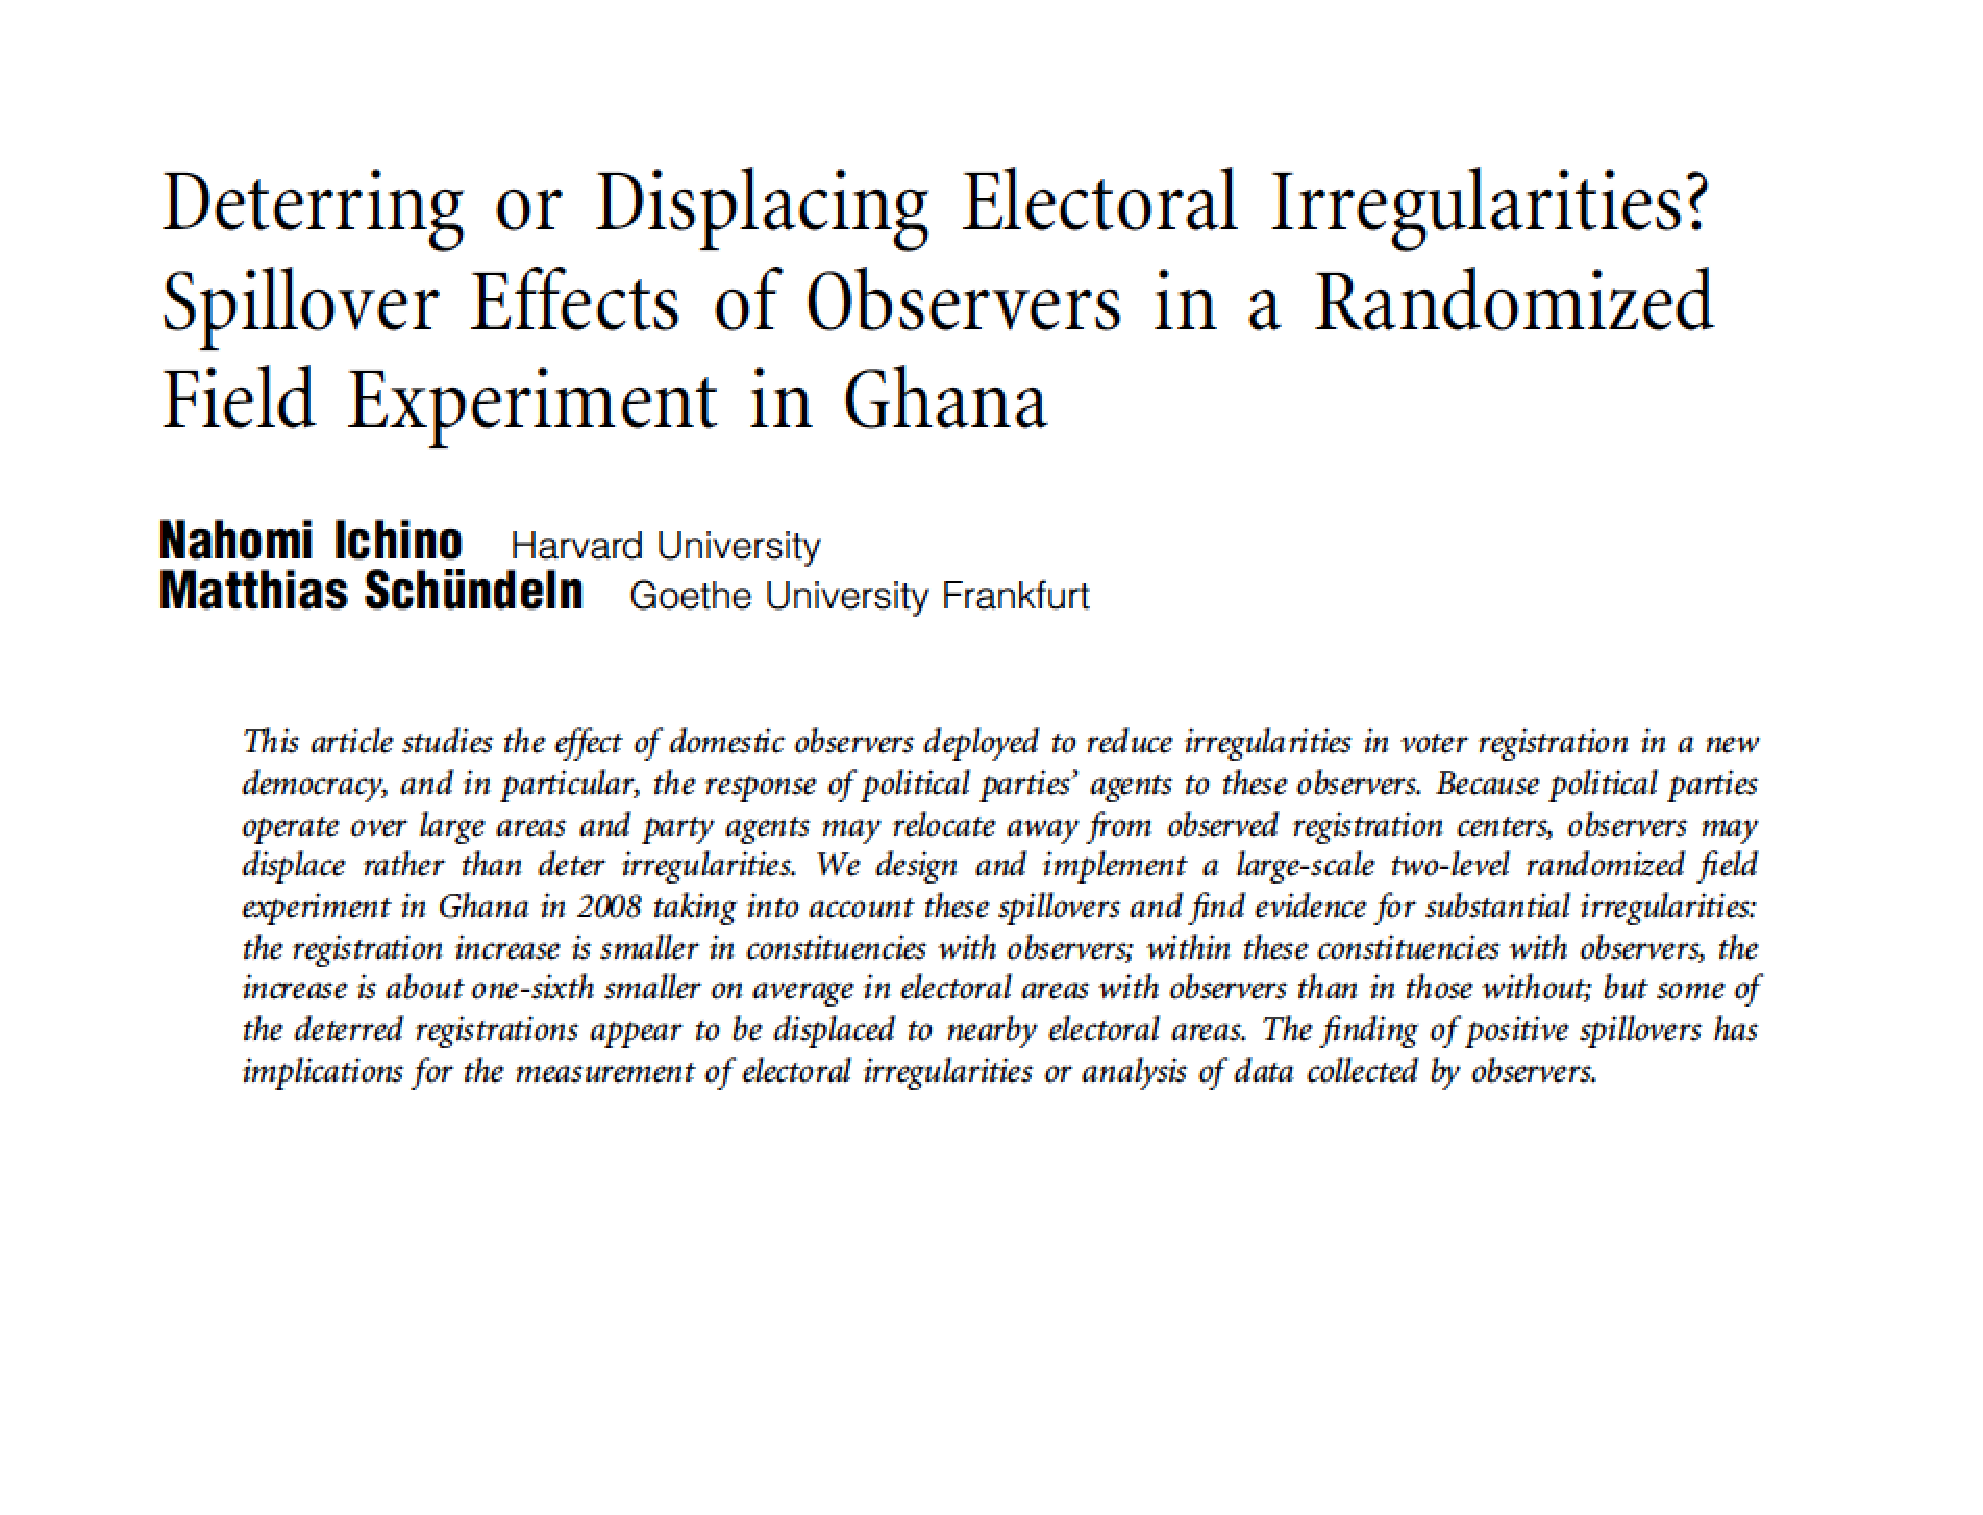
\includegraphics[scale=.35]{pictures/ichinoSchuendeln_title.pdf}
\end{figure}
\end{frame}

\begin{frame}{General questions}
\begin{itemize}
\item What is the research question? \pause
\item What is $M$? \pause
\item Why this $M$? Is it any good?\pause
\item How is \textbf{random assignment} of $M$ being carried out? \pause
\item How is \textbf{control} over confounding observables and unobservables carried out? \pause
\item Which features of the statistical analysis account for observables and unobservables?
\end{itemize}
\end{frame}


\begin{frame}{Question 1(a)}
\begin{itemize}
\item[] (5 marks) The study randomly assign monitors to registration areas and treats smaller increases in registrations (over 2004 levels) at monitored sites (treatment), in contrast to un-monitored sites (control), as evidence of a decrease in fraud. 
Why is change in registrations a good or bad proxy for electoral fraud?
Give 3-4 reasons to justify your answer.
\end{itemize}
\end{frame}

\begin{frame}{Question 1(a)}
Is registration a good or bad proxy for electoral fraud? (Ichino/Sch\"{u}ndeln arguments): \pause
\begin{itemize}
\item Good proxy because: \pause
\begin{itemize}
\item[--] History of manipulations of voter registries $\rightarrow$ more difficult to detect \pause
\item[--] Label ``free and fair'' elections is given when intimidation and vote fraud is absent \pause
\item[--] Unobservable: history of international observers in elections, parties have adapted
\end{itemize}
\end{itemize}
\end{frame}

\begin{frame}{Question 1(a)}
Other arguments. \textbf{Good} because \pause
\begin{itemize}
\item Fake identity easy to obtain in Ghana $\rightarrow$ cheap way for fraud \pause
\item Easy to measure
\item Easy to relate to other measures of voting behavior
\end{itemize}

\textbf{Bad} because \pause
\begin{itemize}
\item Does not account for corrupt election officials \pause -- we would need to know their distribution across control and treatment \pause
\item Can it account for intimidation? \pause
\item Can't catch ballot stuffing \pause $\rightarrow$ although this is rare \pause
\item Relationship between number of registered voters and number of eligible voters in a district? \pause
\item What's the meaning of a change in number of registered voters?
\end{itemize}
\end{frame}

\begin{frame}{Question 1(b)}

\begin{itemize}
\item[] (5 marks) Randomizing instead of permitting the monitors to go wherever they want is designed to permit causal interpretation of the effects. 
Describe the randomization process in detail.
Why would non-random assignment create bias in the estimate of the causal effect of monitors on electoral fraud?
Give at least one reasons each for why the estimated effect may be biased up or down.\\
\end{itemize}
\end{frame}

\begin{frame}{Question 1(b)}
\begin{figure}[H]\centering
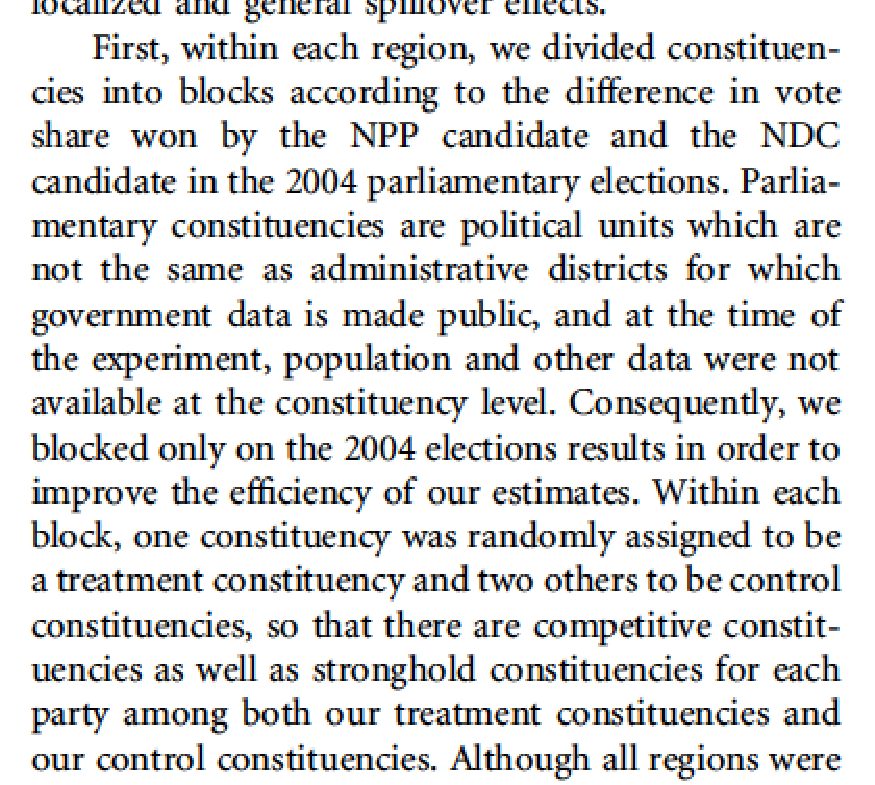
\includegraphics[scale=.5]{pictures/ichinoSchuendeln_randomization.pdf}
\end{figure}
\end{frame}

\begin{frame}{Question 1(b)}
\begin{itemize}
\item Randomization procedure: 
\begin{enumerate} 
\item Blocks of constituencies are generated based on their level of competitiveness (partisan stronghold vs competitive CON) \pause
\item Random assignment of CONs in blocks to treatment ($1/3$) and control ($2/3$) \pause
\item Random assignment of ELAs within each CONs to treatment and control. \pause ELAs in treatment CONs can only be treated (of course) \pause 
\end{enumerate}
\item Without random assignment, characteristics of ELA/CON would not be constant across those which received monitors and those which did not \end{itemize}
\end{frame}

\begin{frame}{Question 1(b)}
\begin{figure}[H]\centering
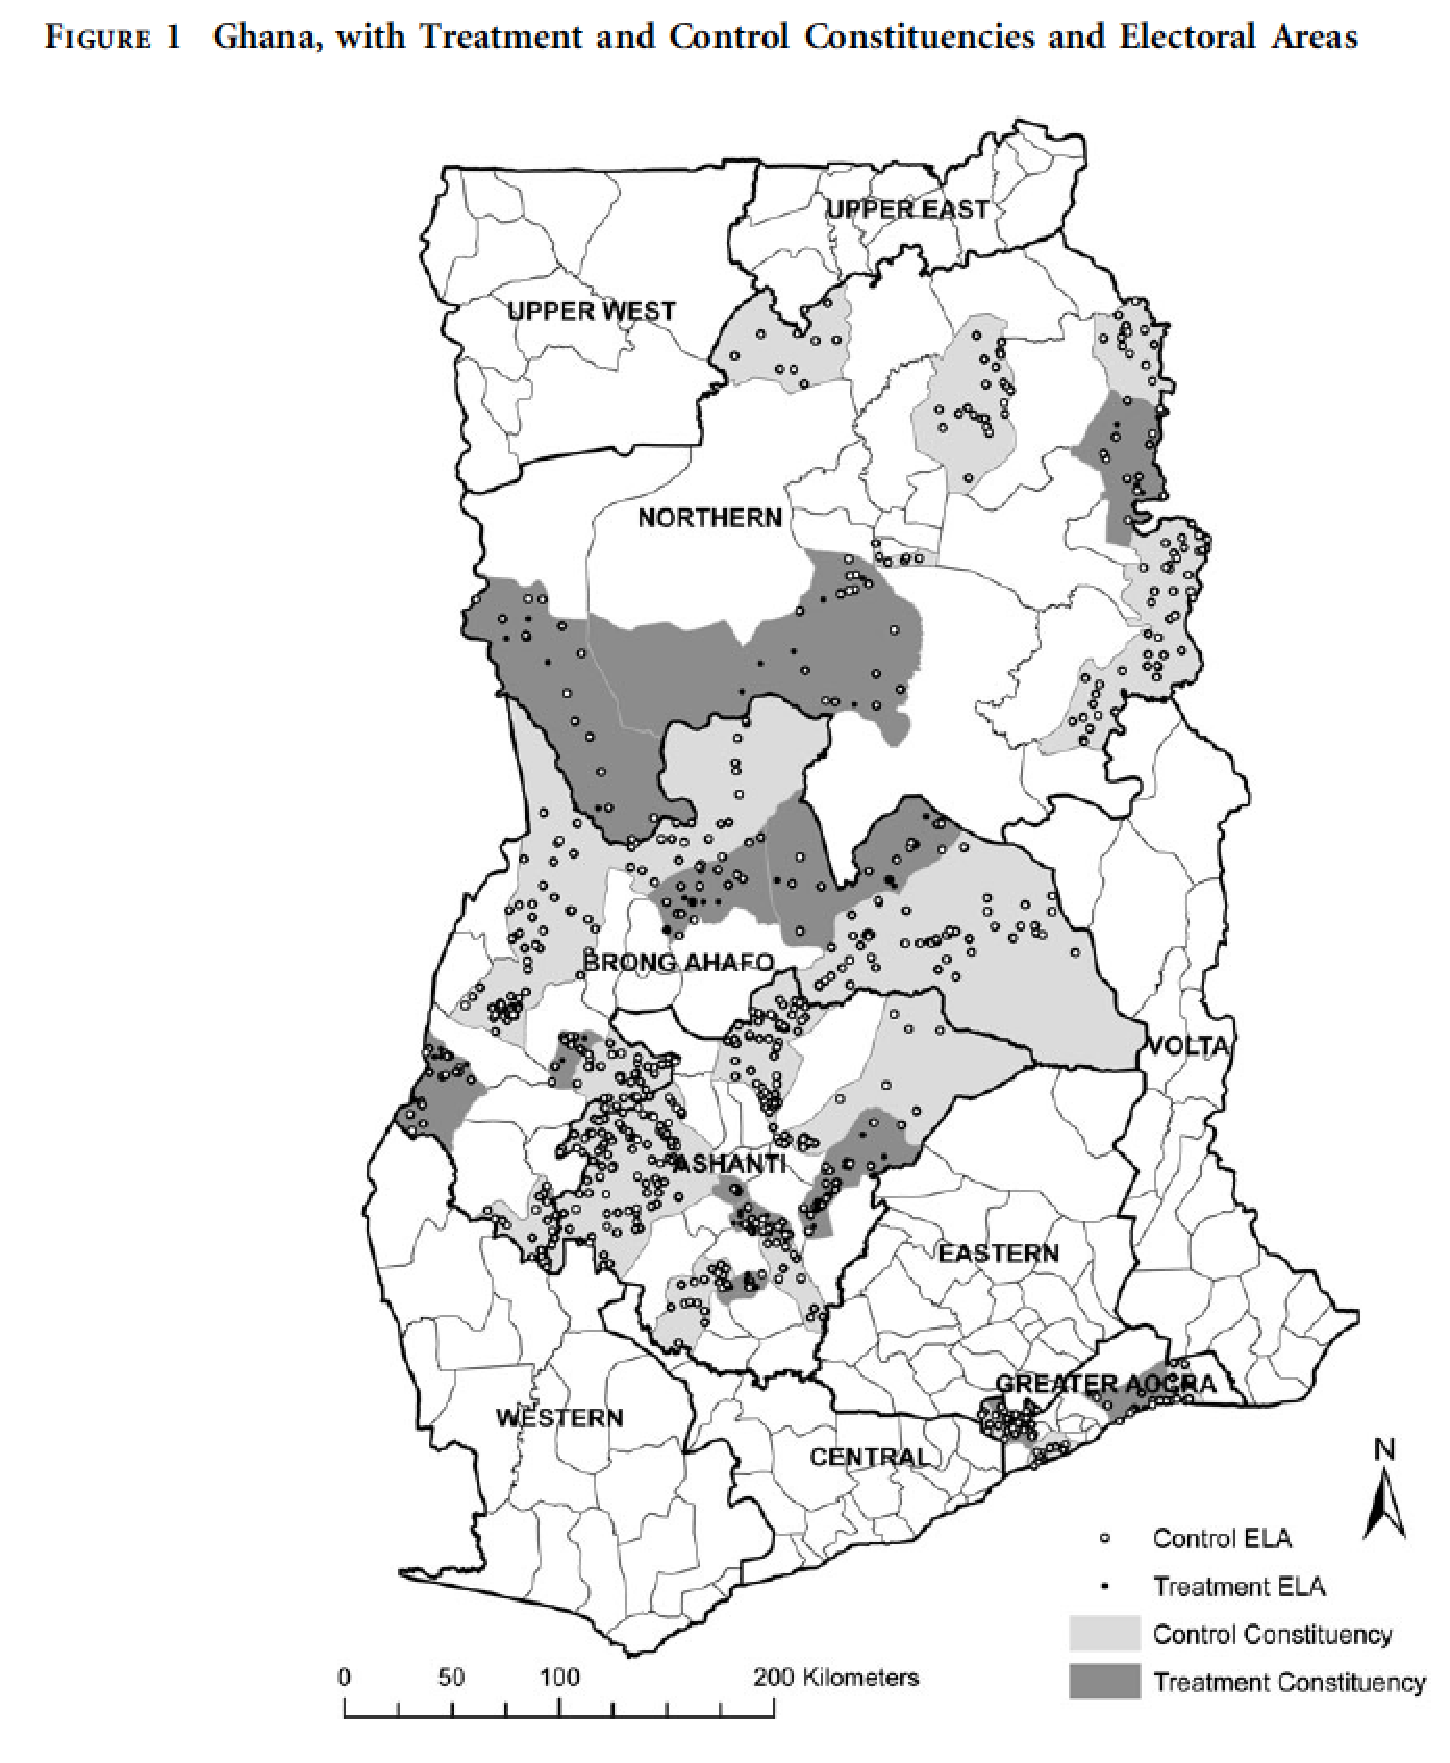
\includegraphics[scale=.25]{pictures/ichinoSchuendeln_map.pdf}
\end{figure}
\end{frame}

\begin{frame}{Question 1(b)}
How good is the the randomization?
\begin{itemize}
\item With no randomization, bias would be any kind of ELA/CON characteristics that make observance more likely. This would bias the causal estimates of monitors on electoral fraud: \pause
\begin{itemize}
\item geography (access to site, density of ELAs/CONs), 
\item ethnic composition of site (in relation to observer if native; unclear effect on treatment effect, could increase intimidation to not commit fraud, underestimate of treatment effect).
\item competitiveness of election at site (ex-ante expectation: more fraud, overestimate of treatment effect) \pause
\end{itemize}
\item By the way: what does this 2-level randomization allow us to measure? \pause -- local and global spill-overs
\end{itemize}

\end{frame}
\begin{frame}{Question 1(b)}
\begin{figure}[H]\centering
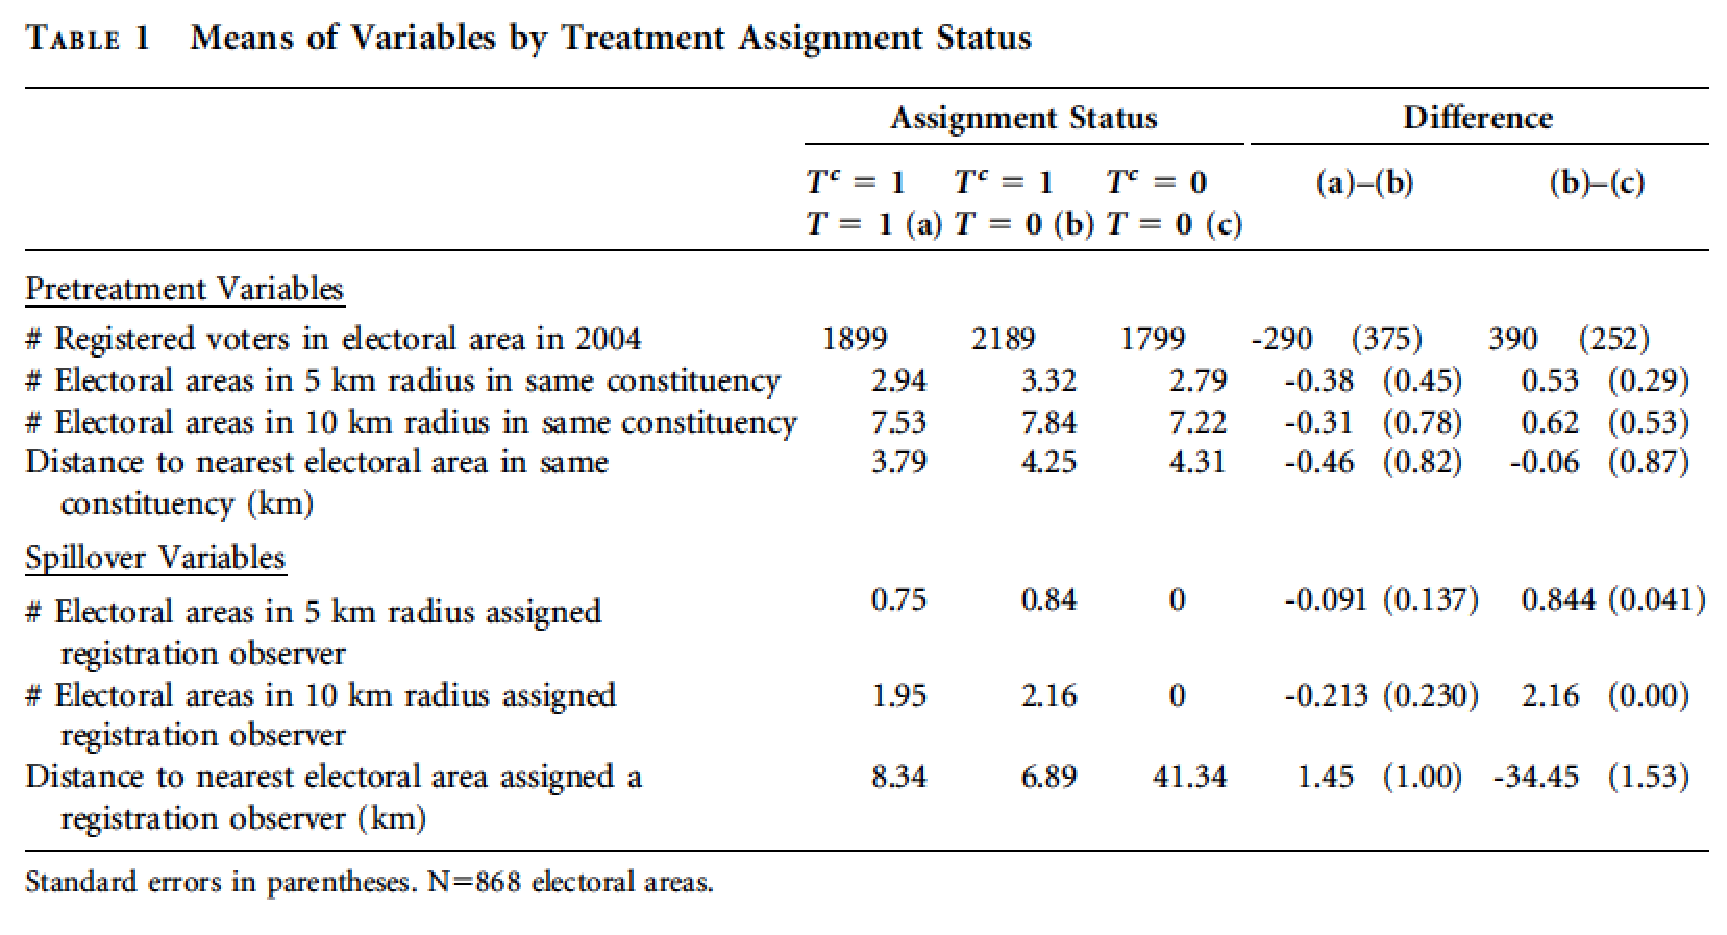
\includegraphics[scale=.37]{pictures/ichinoSchuendeln_balance.pdf}
\end{figure} \pause

Check balance!
\end{frame}

\begin{frame}{Question 1(b)}
\begin{figure}[H]
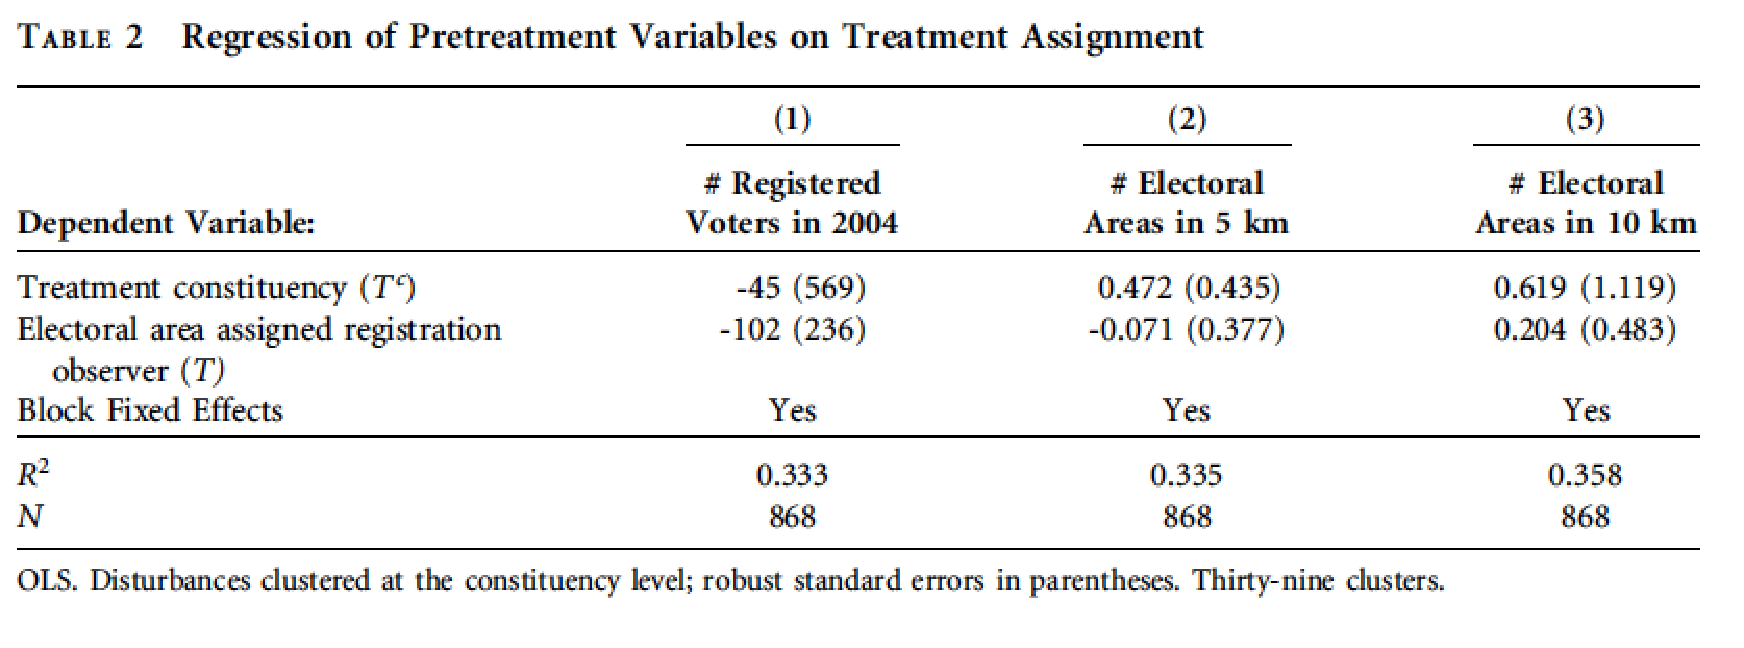
\includegraphics[scale=.37]{pictures/ichinoSchuendeln_preTreatmentOnTreatment.pdf}
\end{figure}\pause

Assess randomization! Pre-treatment effect on changes in registration is 0!
\end{frame}

\begin{frame}{Question 1(c)}

\begin{itemize}
\item[] (5 marks) Load ``ghana.dta.''
The outcome variable in this dataset is the percent change in registration from the election in 2004 to the election 2008 for each electoral area (ELA), ``percchangeregELA0804''. 
You are also given an indicator for whether observers where assigned to the ELA (``Tela'') and whether they visited the ELA (``Vela'').
What is the treatment in this experiment? 
What is the manipulation in this experiment? 
Is the manipulation used here a good proxy for the treatment? 
Use variables ``Vela'' and ``Tela'' to assess whether the manipulation is any good. 
What could be reasons for a failure to treat?
\end{itemize}
\end{frame}

\begin{frame}[fragile]{Question 1(c)}
\begin{lstlisting}
tab Tela Vela

           |   =1 if visited ELA
 =1 if ELA |  during registration
  assigned |  (based on observer
        to |       reports)
 treatment |         0          1 |     Total
-----------+----------------------+----------
         0 |       766         25 |       791 
         1 |        12         65 |        77 
-----------+----------------------+----------
     Total |       778         90 |       868 
	
\end{lstlisting}
We have 15\% of cases where ``Tela'' is not equal to ``Vela'' in the treatment group (12 out of 77). 
The paper reports on difficulties to reach sites during rainy season.
\end{frame}

\begin{frame}{Question 1(d)}
(3 marks) Regress percent change in registrations on the treatment variable, that is, pick one of ``Vela'' or ``Tela'' as your independent variable. 
Explain why you would use one or the other as your operationalization of the treatment in this regression. 
Report and interpret the result. \pause

You had to report and interpret regression results, answer needs argument for either Tela or Vela and needs to mention the coefficient on Tela/Vela and the result of the hypothesis test over the coefficient of Tela/Vela. \pause

Let's see what you did!
\end{frame}


\begin{frame}{Question 1(d)}
\begin{figure}[H]\centering
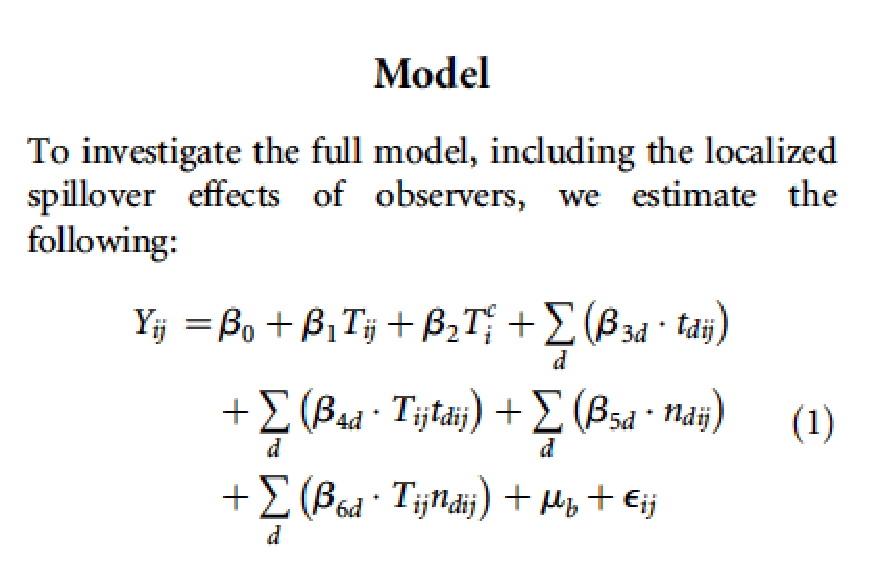
\includegraphics[scale=.7]{pictures/ichinoSchuendeln_statsModel.pdf}
\end{figure}
\end{frame}


\begin{frame}{Question 1(d)}
\begin{itemize}
\item Outcome: $Y_{ij}$ = percentage change in number of registered voters from 2004 to 2008 in ELA $j$ and CON $i$ \pause
\item $M$ and $M^c$ (here referred to as $T$ and $T^c$) = assignment of observers to ELA and CON \pause
\item Spillover variables  \pause -- ensuring that the Stable Unit Treatment Variable Assumption (SUTVA) is met
\end{itemize}
\end{frame}

\begin{frame}{Question 1(e)}
\begin{itemize}
\item[] Question 1(e): (5 marks) Regress percent change in registrations on the indicator for whether an area was monitored and the number of monitored areas within 5km.
The data set contains variables indicating the number of assigned monitors in ELAs within 5km (``assignedTin5C'') and the number of monitors visiting ELAs within 5km (``visitedin5C'').
Pick one of those variables depending on which variable you chose in (d) to operationalize the treatment (``Vela'' or ``Tela''). 
Interpret the result. 
What does this result tell us about how political parties responded to the presence of electoral monitors?
\end{itemize}
\end{frame}

\begin{frame}{Question 1(e)}
\begin{figure}[H]\centering
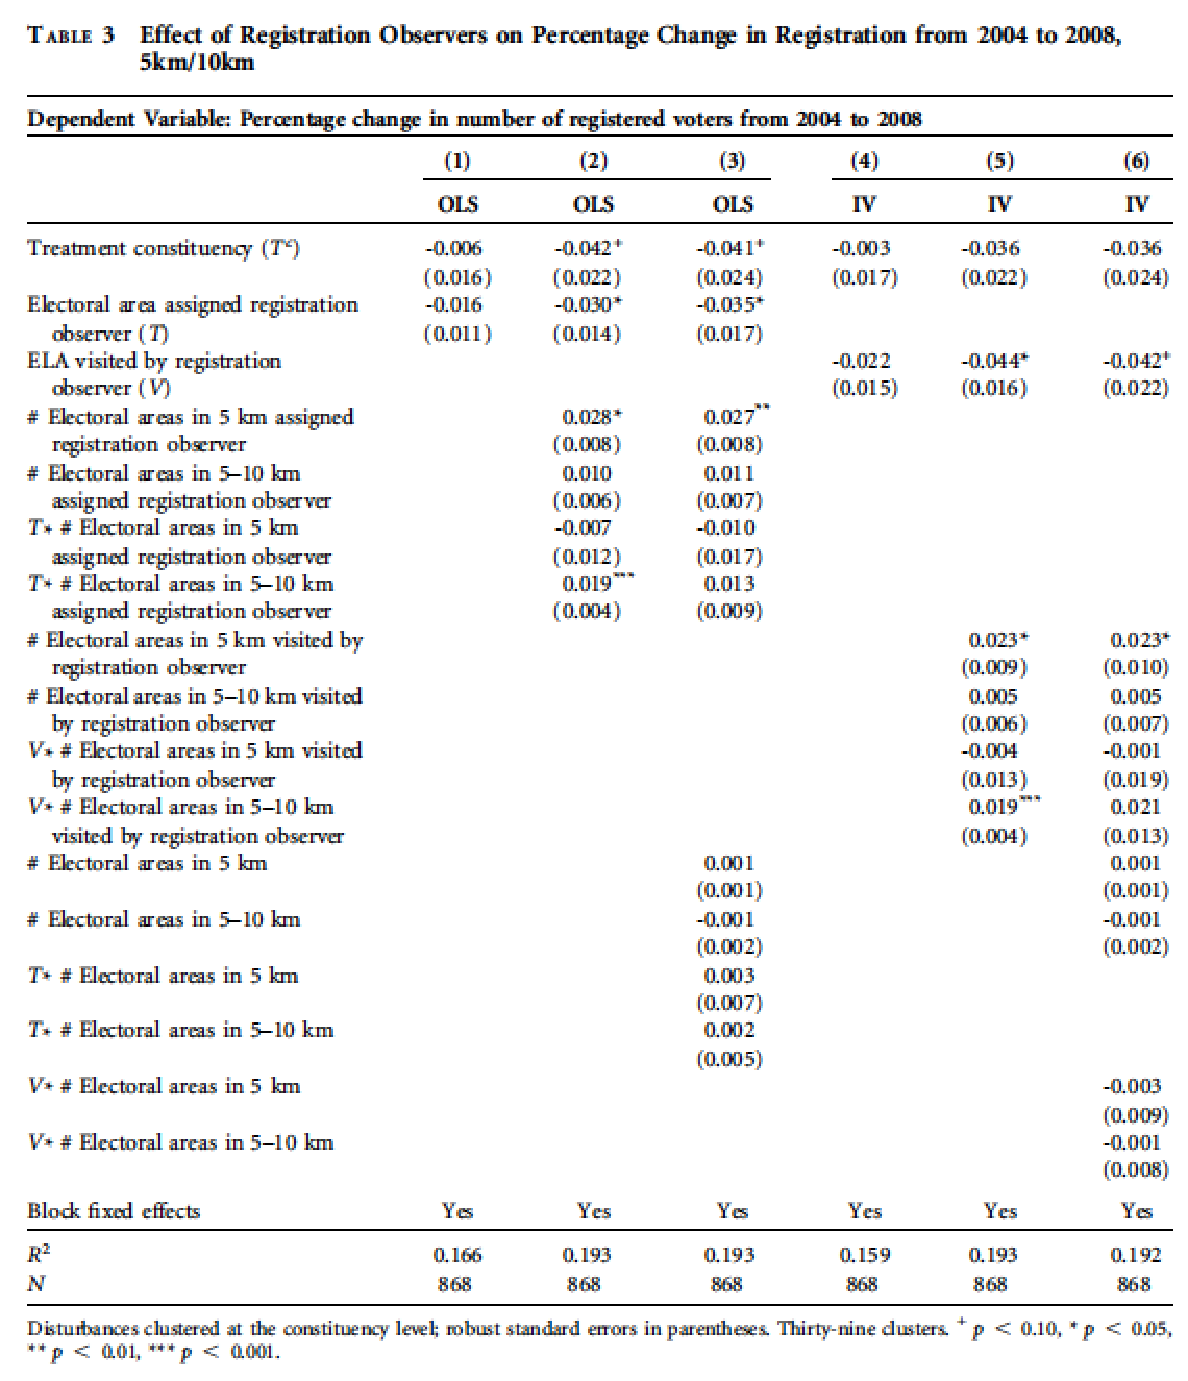
\includegraphics[scale=.35]{pictures/ichinoSchuendeln_results.pdf}
\end{figure}
\end{frame}

\begin{frame}{Question 1(e)}
\begin{itemize}
\item Report and interpret regression results (complete mentioning of coefficient estimates, hypothesis test over the coefficient). \pause
\item The variable ``assignedTin5C'' allows to talk about spill-overs to nearby ELAs. \pause
\item This gives us an indication of whether parties focussed their fraud activity on nearby ELAs as soon as observers showed up.
\end{itemize}
\end{frame}

\begin{frame}{Noteworthy elements of the statistical model and experiment}
\begin{itemize}
\item Controlling for fixed effects within blocks \pause -- simply include a variable that indicates in which block an observation (ELA) resides \pause
\item Allow for correlation between errors within constituency \pause -- we will learn the math behind this when we talk about hierarchical models. \pause $\rightarrow$ Intuitively, is what we have seen with serial correlations! \pause
\item Measure non-compliance (assigned to receive observer vs observer visited)
\end{itemize}

\end{frame}

\begin{frame}{Question 1(f)}
Question 1(f): (2 marks) Discuss in 2-3 sentences what we learn from this about the effects of election monitoring. \pause

Could be displacement and not just deterrence (which is also the conclusion of the paper itself).
\end{frame}


\begin{frame}{Question 1(g)}
\begin{itemize}
\item[] Question 1(g): (5 marks) Explain how the experiment and analysis of experimental data presented in this paper helps to meet the Stable Unit Treatment Variable Assumption (SUTVA).
\end{itemize}
\end{frame}

\begin{frame}{Question 1(g)}
\begin{itemize}
\item Recall what SUTVA says and let's evaluate what the experiment does to meet SUTVA: \pause
\begin{enumerate}
\item $T_i$ only affects $i$  $\rightarrow$ no spill-overs: This study acknowledges that spill-over effects necessarily exist and tackles them through random assignment of observers to CON and then within treatment CON to ELAs (two-step randomization). The resulting indicators of observers in nearby ELAs of varying distance and nearby CON allows to measure the spillover effects. \pause
\item effect of $T_i$ homogenous among subjects: not debated \pause
\item $T_i$ is invariant with respect to mechanism by which $T_i$ is provided: not debated \pause
\item all possible states of the world are observed: registration as proxy for electoral fraud gives us observable measures of treatment and control group
\end{enumerate}
\end{itemize}
\end{frame}


\begin{frame}{Question 1(g)}
\begin{itemize}
\item Recall what SUTVA says and let's evaluate what the experiment does to meet SUTVA (continue): \pause 
\begin{enumerate}
\item[5.] no interaction between $Y_i$ and $T_i$: \pause It may be that the registration data itself is subject to fraud but authors argue it is not. \pause $Y_i$ may determine $T_i$, that is, the extend of fraud in an ELA may affect the ability of researchers to assign observers to an ELA (or the willingness of observers to actually go to that ELA). \pause Authors claim they take care of such variation through random assignment but we know from comparing ``Tela'' and ``Vela'' that there may be a problem here. 
\end{enumerate}
\end{itemize}
\end{frame}


\begin{frame}{Question 1(h)}
Question 1(h): (5 marks) What is blocked randomization, how is it used in this experiment, and how does it improve the estimate of the causal effect of monitoring on electoral fraud?\pause
\begin{itemize}
\item Blocked randomization means that treatment and control are randomly assigned within blocks (sub-samples sharing the same characteristics) and not within the full sample. 
\item In this study, researchers blocked on 2004 election result.
\item They separate CONs in whether they had competitive or non-competitive elections in 2004 and randomly assigned to treatment and control within the set of competitive CONs and then again within the set of non-competitive CONs. 
\item Done to alleviate the influence competitive election potentially has on the treatment effect
\end{itemize}
\end{frame}

\begin{frame}{Question 2(a)}
(5 marks) What is the research question, the dependent variable (Y), the experimental manipulation (M), and the intended treatment (T)? \pause

Are partisan messages effective in mobilizing turnout? \pause Y: Turnout, M: partisan/non-partisan made salient in a message delivered via phone call, T: delivering a partisan message
\end{frame}

\begin{frame}{Question 2(b)}
(7 marks) In an ideal experiment, the experimenter would manipulate the partisan identity of subjects directly (i.e., randomly assign subject $i$ to be either Republican or Democrat). 
Why is this not possible? How is the author dealing with this issue in implementing the presented experiment, i.e. what is his manipulation? \pause

\begin{itemize}
\item Partisanship emerges from socialization: impossible to replicate given limited resources. \pause 
\item The author manipulates the salience of partisanship and hopes the effect is strong enough to enter subjects' considerations. \pause 
\item The experiment has no control over whether subjects actually pick up on the partisan prime
\end{itemize}
\end{frame}

\begin{frame}{Question 2(c)}
(8 marks) Which observables is the author controlling for in this study and how is he implementing these controls in experimental design and statistical analysis? \pause

\begin{itemize}
\item Dummies for turnout in the past in the statistical model \pause
\item In the experimental design, the author includes Dem and Rep messages to control for potential differences in the treatment effect across groups of partisans \pause
\item Also, randomization is done by blocking on past turnout and only applied to partisans
\end{itemize}
\end{frame}

\begin{frame}{Question 3}
Unlike in observational studies, experiments allow the researcher to decide how many people will participate. 
The research will have to calculate how many people s/he needs to uncover a significant effect of the treatment on the outcome variable. 
S/he trie to assess the statistical power of the statistical test used in analyzing the data generated by an experiment. 
Recall what ``power of a statistical test'' means (Week 7, slide 32)
\end{frame}

\begin{frame}{Question 3(a)}
(5 marks) By statistical power, we refer to $P(\text{Reject the null hypothesis}|\text{Null hypothesis is false})$. 
How exactly is this different than statistical significance of a test? \pause Can you think of why statistical power is a less well defined problem than statistical significance? \pause

The level of significance of a test is the $P(\text{Reject the null hypothesis}|\text{Null hypothesis is true})$ \pause The event ``the null hypothesis is false'' is much harder to define than the event ``the null hypothesis is true'' (we don't really know what is out there in the world)
\end{frame}

\begin{frame}{Question 3(b)}
There is an obvious tradeoff between statistical power and costs of a study. Why is this the case? Why would you want a sample as large as you can afford because of statistical power? Explain the relationship between sample size and statistical power. \pause

Larger samples give more reliable results, a smaller variance of the estimated of the statistic of interest, and small samples often leave the null hypothesis unchallenged even if the null hypothesis is not true.
\end{frame}

\begin{frame}{Question 3(c)}
Read the experiment (link) and explain in your words how the researchers assess whether their experiment will have enough statistical power. What is the metric by which they judge whether it has enough statistical power? \pause

The metric is whether the sample size is large enough to see a significant effect in the applied hypothesis test at 80\% power \pause

See R file for a power analysis
\end{frame}


\frame{
\frametitle{Conclusion}
\begin{center}
All clear? More questions? \\
Thanks and see you next week!
\end{center}
}

\end{document}